\documentclass{beamer}

\setbeamertemplate{navigation symbols}{}
\setbeamertemplate{footline}[15]
\setbeamercolor{title}{fg=white,bg=darkred!80!black}
\usetheme{CambridgeUS}

\title[ParsEvalMPI]{ParsEvalMPI: comparison of gene structure annotations in parallel}
\author{Daniel S. Standage}
\date{\today}
\institute[BCB]{Bioinformatics and Computational Biology}

\begin{document}
 

\begin{frame}
  \titlepage
\end{frame}

\section{Background}
\subsection{Gene prediction (annotation)}
\begin{frame}
  \frametitle{Gene prediction (annotation)}
  {\LARGE Input}
  \hrule
  \vspace{5px}
  String representing DNA sequence
  
  \vspace{30px}
  
  {\LARGE Output}
  \hrule
  \vspace{5px}
  Regions (coordinates) of sequence that correspond to genes and their structural components
\end{frame}

\subsection{Comparing annotations}
\begin{frame}
  \frametitle{Comparing annotations}
  \begin{center}
    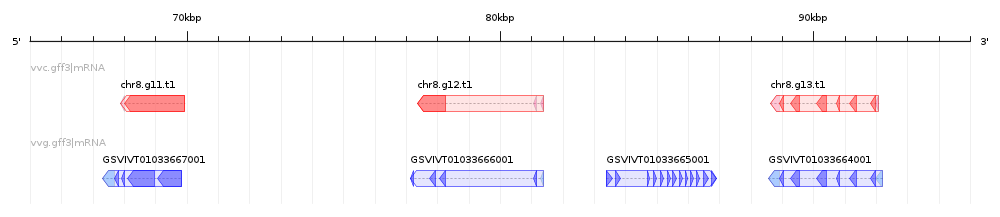
\includegraphics[width=325px]{predictions.png}
  \end{center}
\end{frame}

\section{Program overview}
\subsection{ParsEval in Perl}
\begin{frame}
  \frametitle{Previous implementation}
  { \LARGE ParsEval }
  \vspace{1px}
  \hrule
  \vspace{10px}
  
  \begin{itemize}
    \item<1-> written in Perl
    \item<2-> external dependencies (platform-specific)
    \item<3-> significant memory demands
    \item<4-> serial execution: run time in minutes to hours
  \end{itemize}
\end{frame}

\subsection{ParsEvalMPI in C}
\begin{frame}
  \frametitle{New implementation}
  { \LARGE ParsEvalMPI }
  \vspace{1px}
  \hrule
  \vspace{10px}

  \begin{itemize}
    \item<1-> written in C
    \item<2-> external dependencies (cross-platform)
    \item<3-> reduced memory demands
    \item<4-> parallel execution: run time in ...
  \end{itemize}
\end{frame}

\subsection{Program overview}
\begin{frame}
  \frametitle{Program overview}
  \begin{itemize}
    \item<2-> delegation
    \item<3-> local analysis
    \item<4-> global analysis
  \end{itemize}
\end{frame}

\subsection{Delegation}
\begin{frame}
  \frametitle{Delegation}
  \begin{center}
    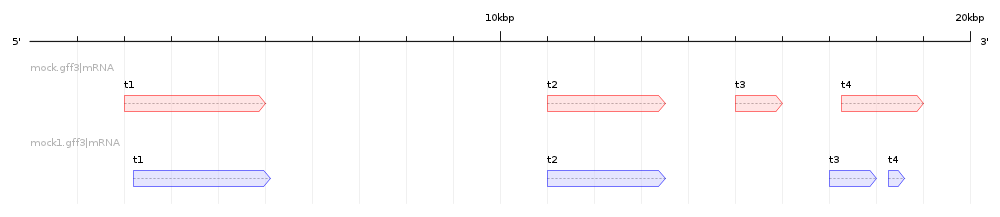
\includegraphics[width=325px]{mock.png}
  \end{center}
  \invisible{\begin{enumerate}
    \item all data on all processors
    \item even distribution of DNA
    \item even distribution of genes
    %\item even distribution of combined gene length
  \end{enumerate}}
\end{frame}

\begin{frame}
  \frametitle{Delegation}
  \begin{center}
    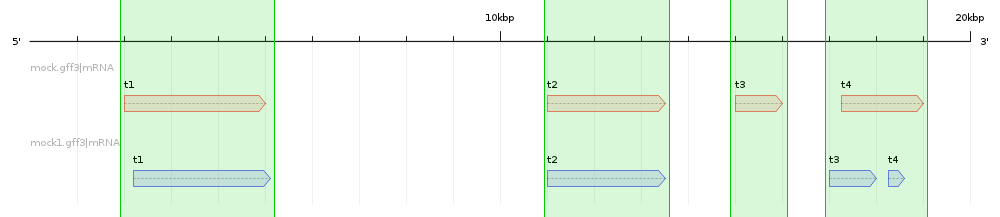
\includegraphics[width=325px]{data.png}
  \end{center}
  \begin{enumerate}
    \item<2-> all data on all processors
    \item<3-> even distribution of DNA
    \item<4-> even distribution of genes
    %\item<5-> even distribution of combined gene length
  \end{enumerate}
\end{frame}

\subsection{Local and global analysis}
\begin{frame}
  \frametitle{Local and global analysis}
  \begin{itemize}
    \item<1-> Local analysis
    \begin{itemize}
      \item<2-> generate local model vector
      \item<3-> send local vector to global vector on root processor
      \item<4-> analyze local vector, print scores
    \end{itemize}
    \item<1-> Global analysis
      \begin{itemize}
        \item<5-> receive local vectors from each processor
        \item<6-> analyze combined global vector, print scores
      \end{itemize}
  \end{itemize}
\end{frame}

\section{Evaluation}
\subsection{Load balancing}
\begin{frame}
  \frametitle{Load balancing}
  \begin{center}
    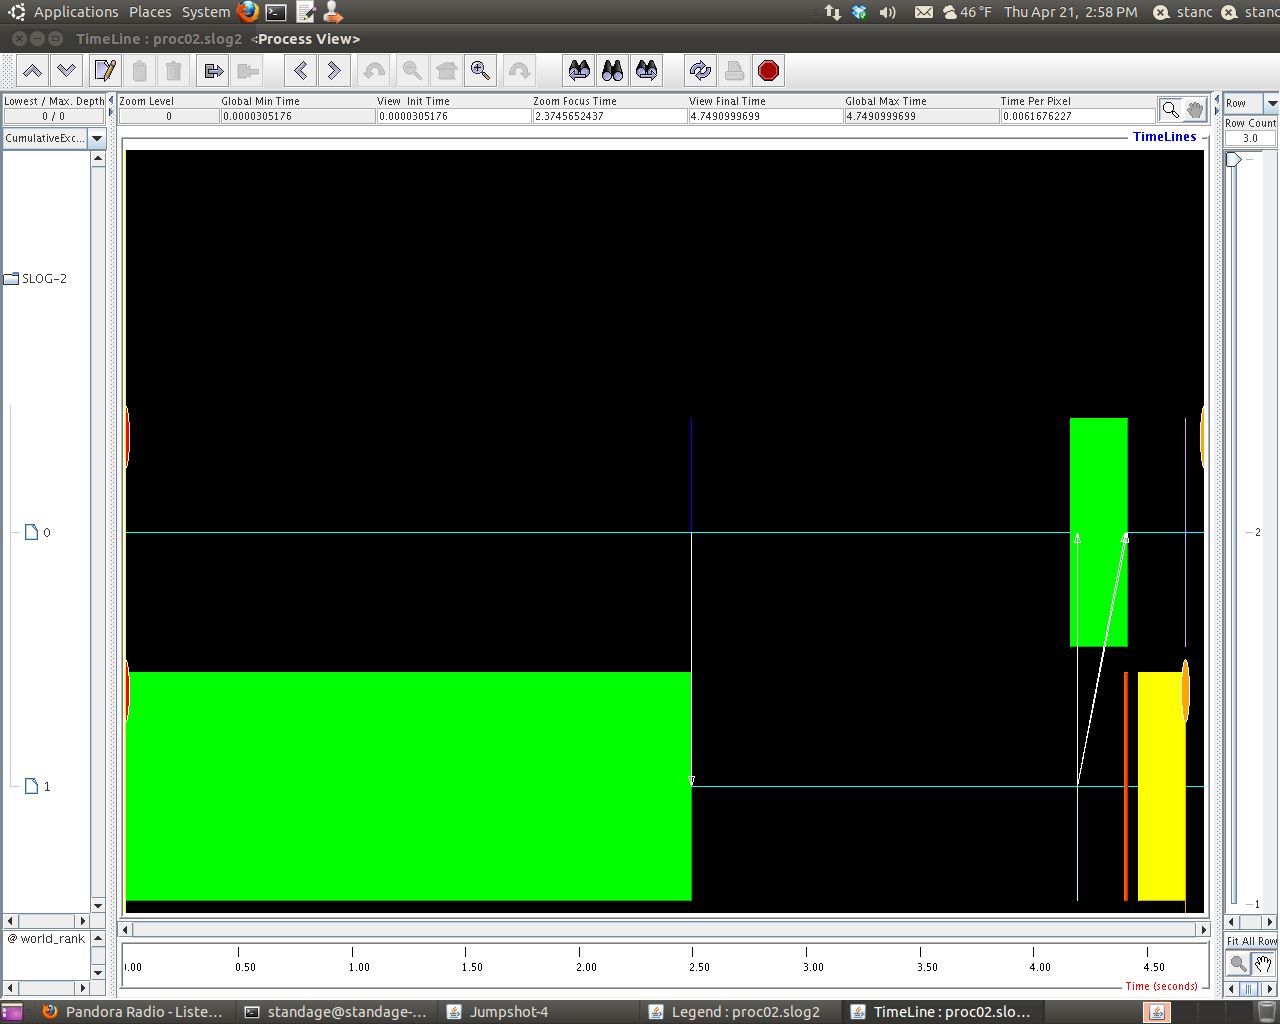
\includegraphics[height=200px]{procs-02.png}
  \end{center}
\end{frame}
\begin{frame}
  \frametitle{Load balancing}
  \begin{center}
    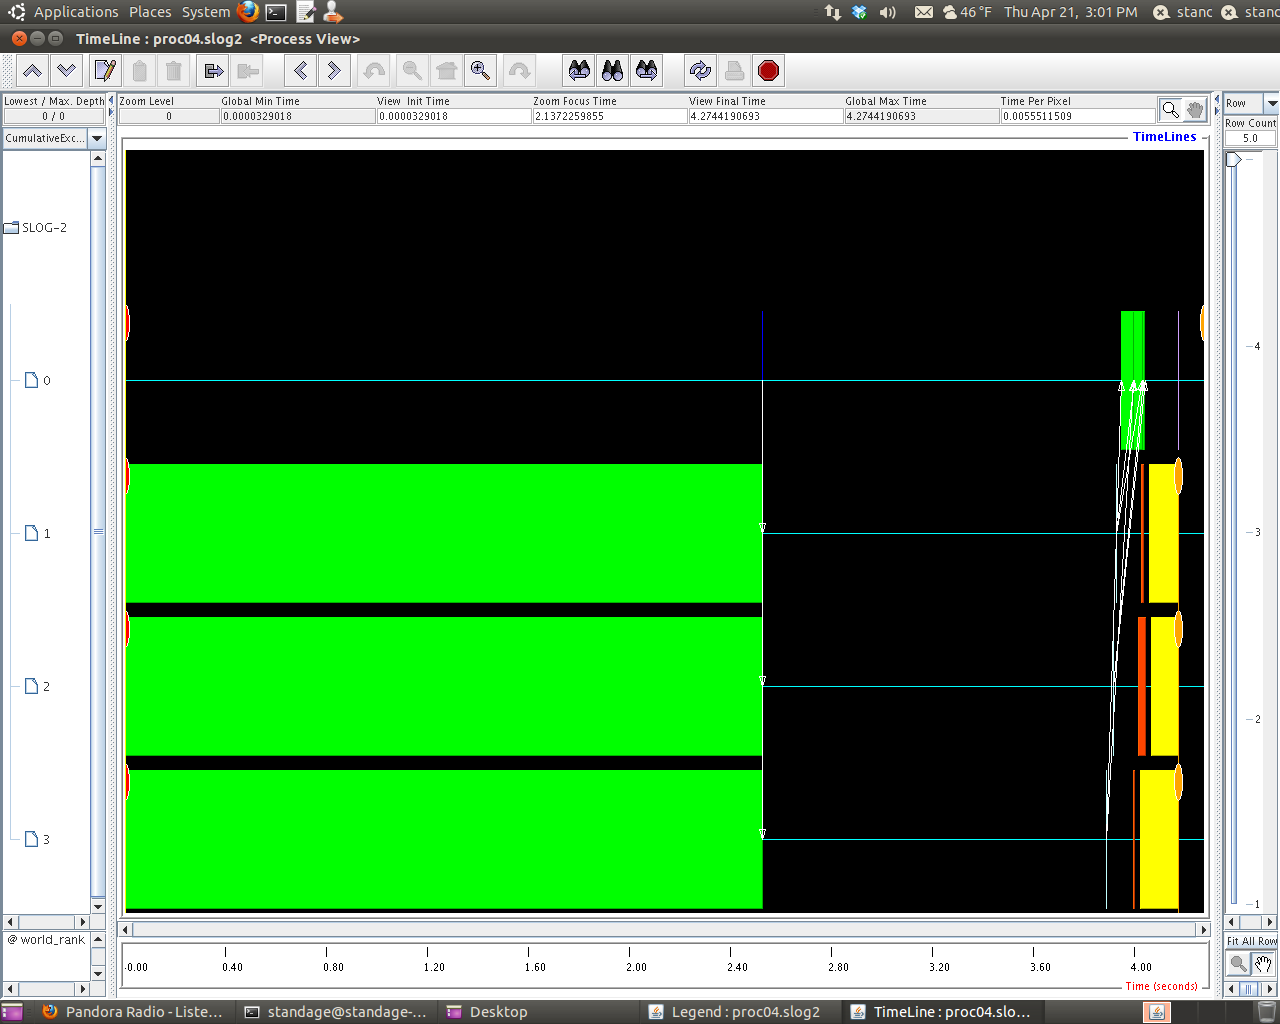
\includegraphics[height=200px]{procs-04.png}
  \end{center}
\end{frame}
\begin{frame}
  \frametitle{Load balancing}
  \begin{center}
    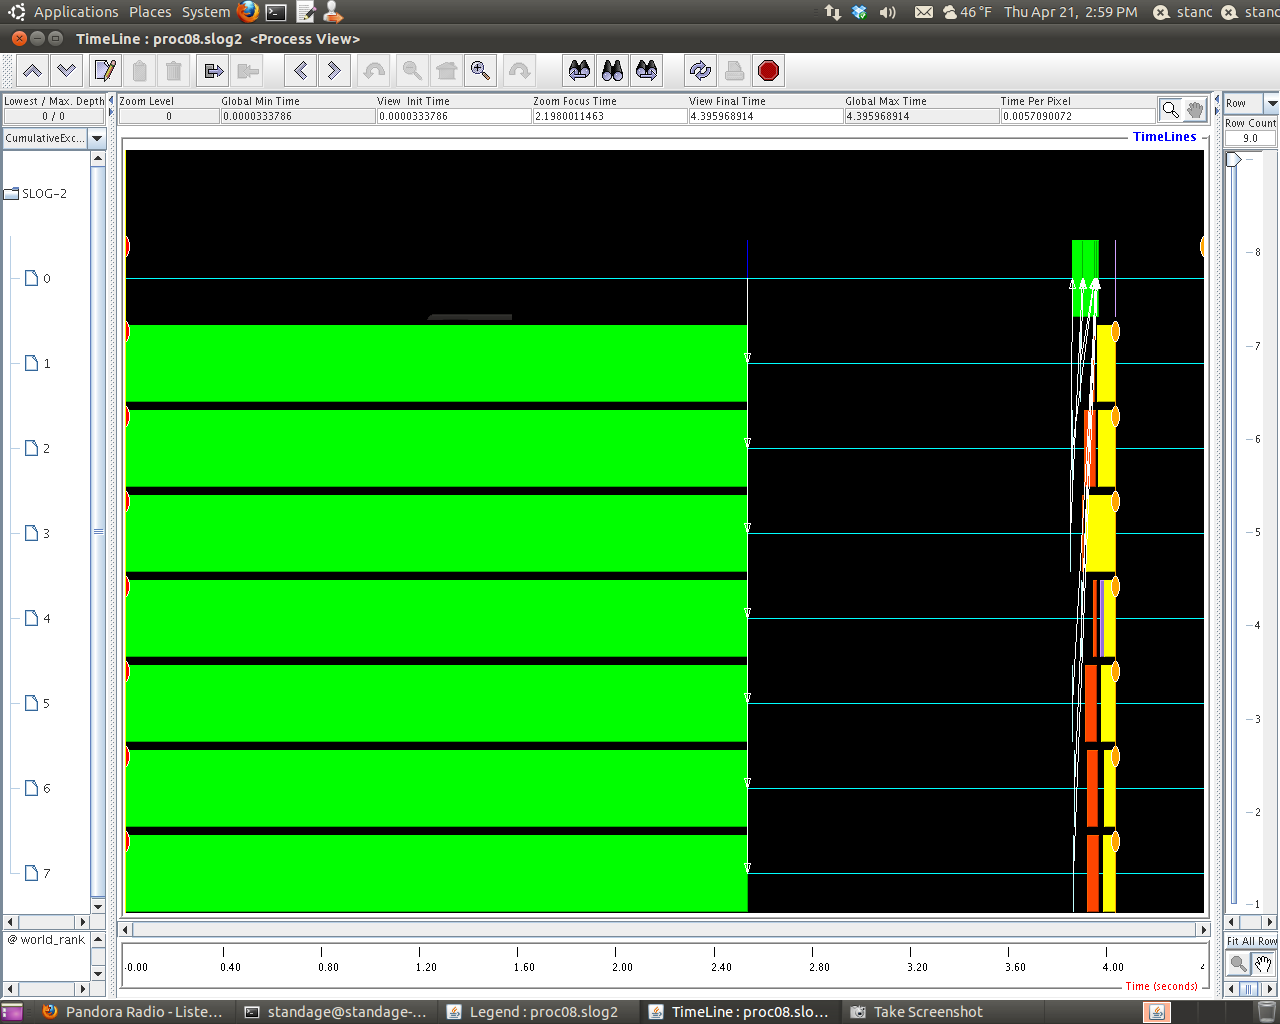
\includegraphics[height=200px]{procs-08.png}
  \end{center}
\end{frame}

%\begin{frame}
%  \frametitle{Load balancing}
%  \begin{center}
%    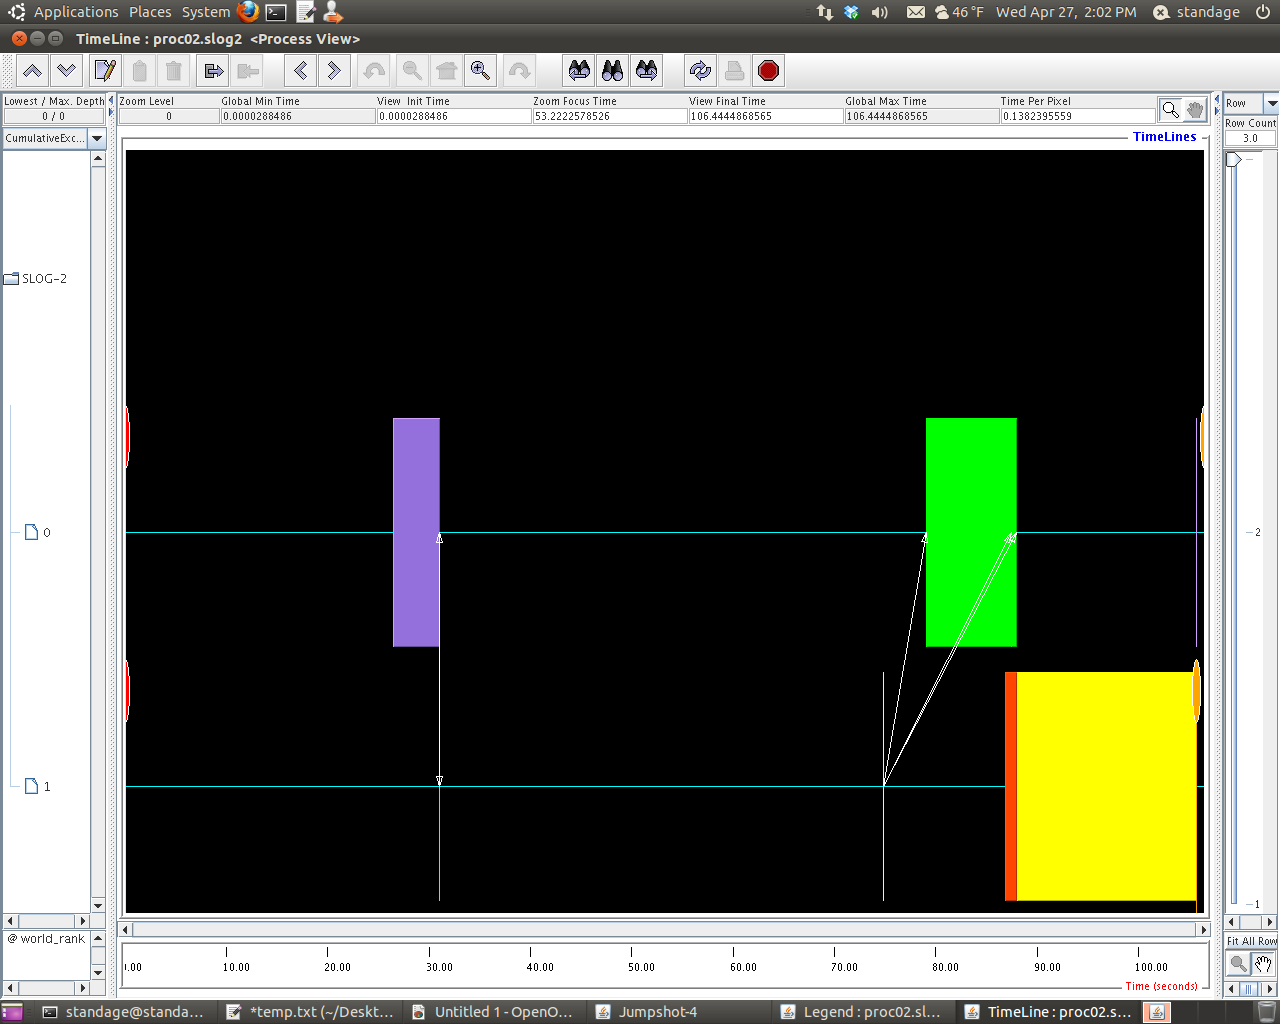
\includegraphics[height=200px]{proc02-hg.png}
%  \end{center}
%\end{frame}
\begin{frame}
  \frametitle{Load balancing}
  \begin{center}
    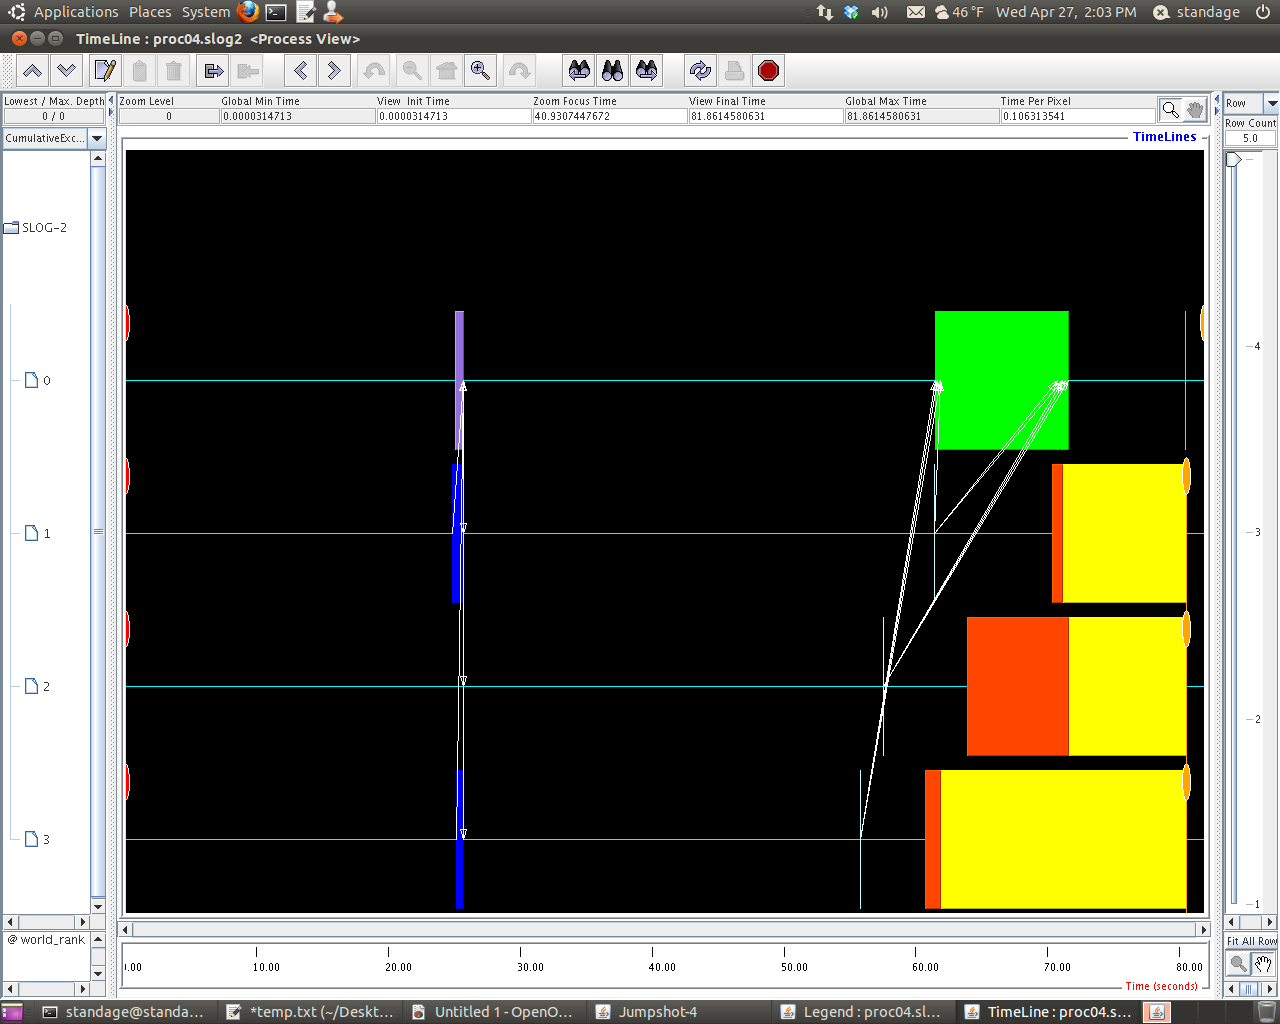
\includegraphics[height=200px]{proc04-hg.png}
  \end{center}
\end{frame}
\begin{frame}
  \frametitle{Load balancing}
  \begin{center}
    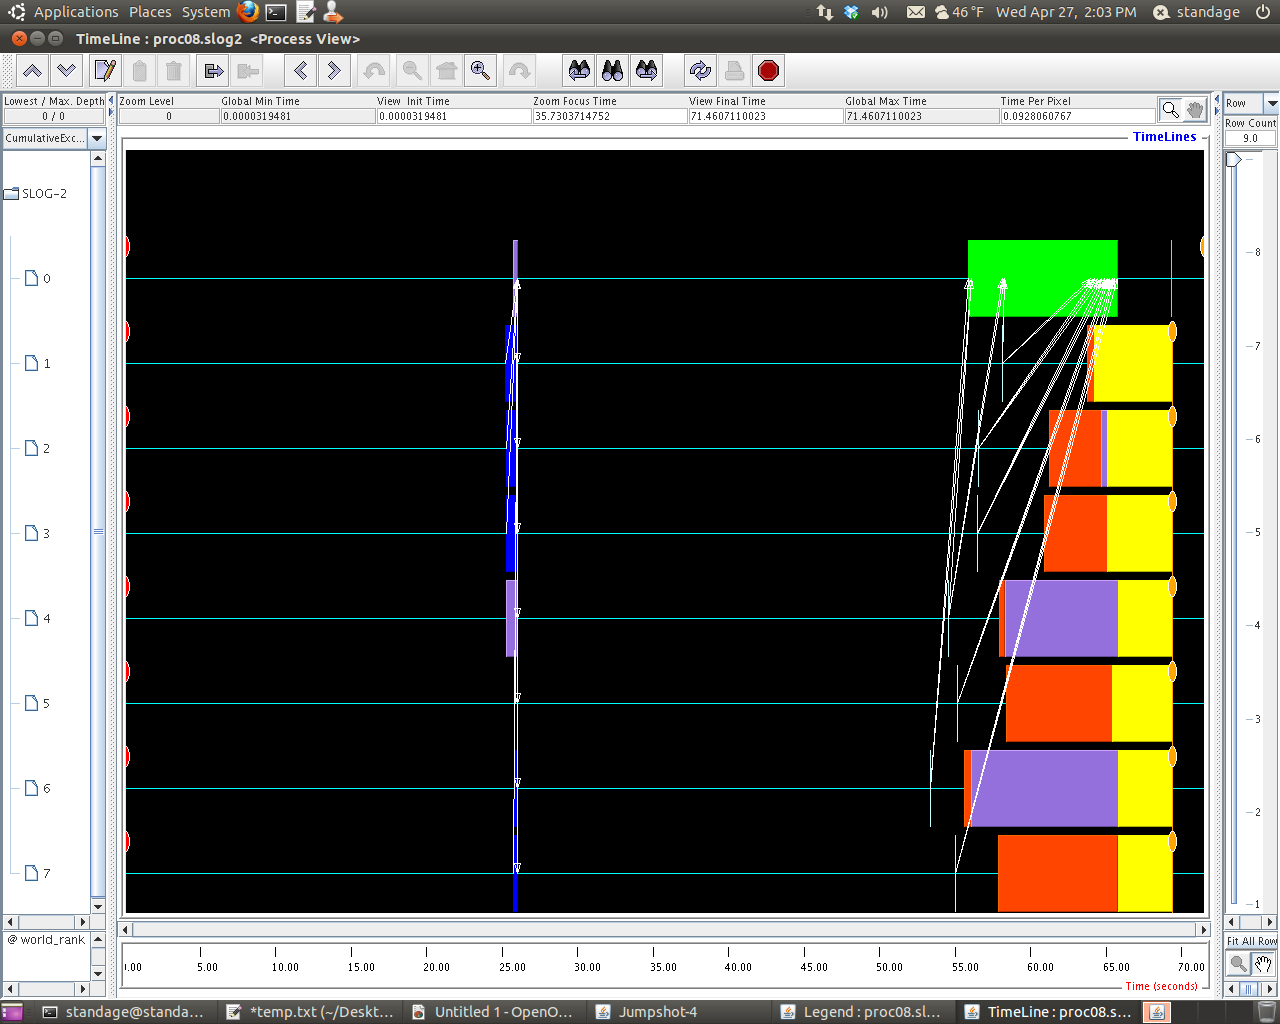
\includegraphics[height=200px]{proc08-hg.png}
  \end{center}
\end{frame}
\begin{frame}
  \frametitle{Load balancing}
  \begin{center}
    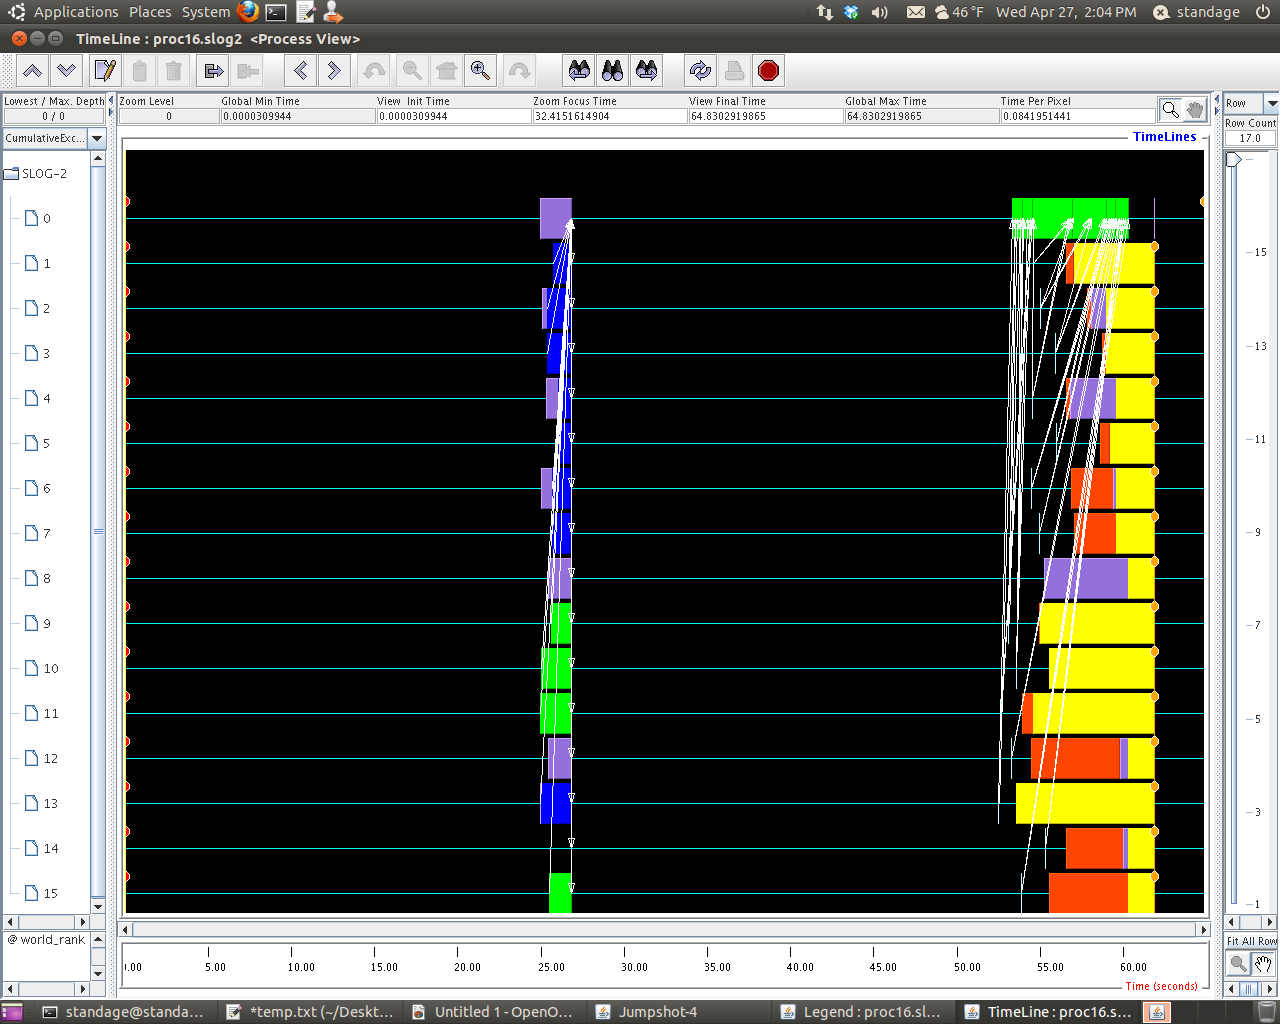
\includegraphics[height=200px]{proc16-hg.png}
  \end{center}
\end{frame}
\begin{frame}
  \frametitle{Load balancing}
  \begin{center}
    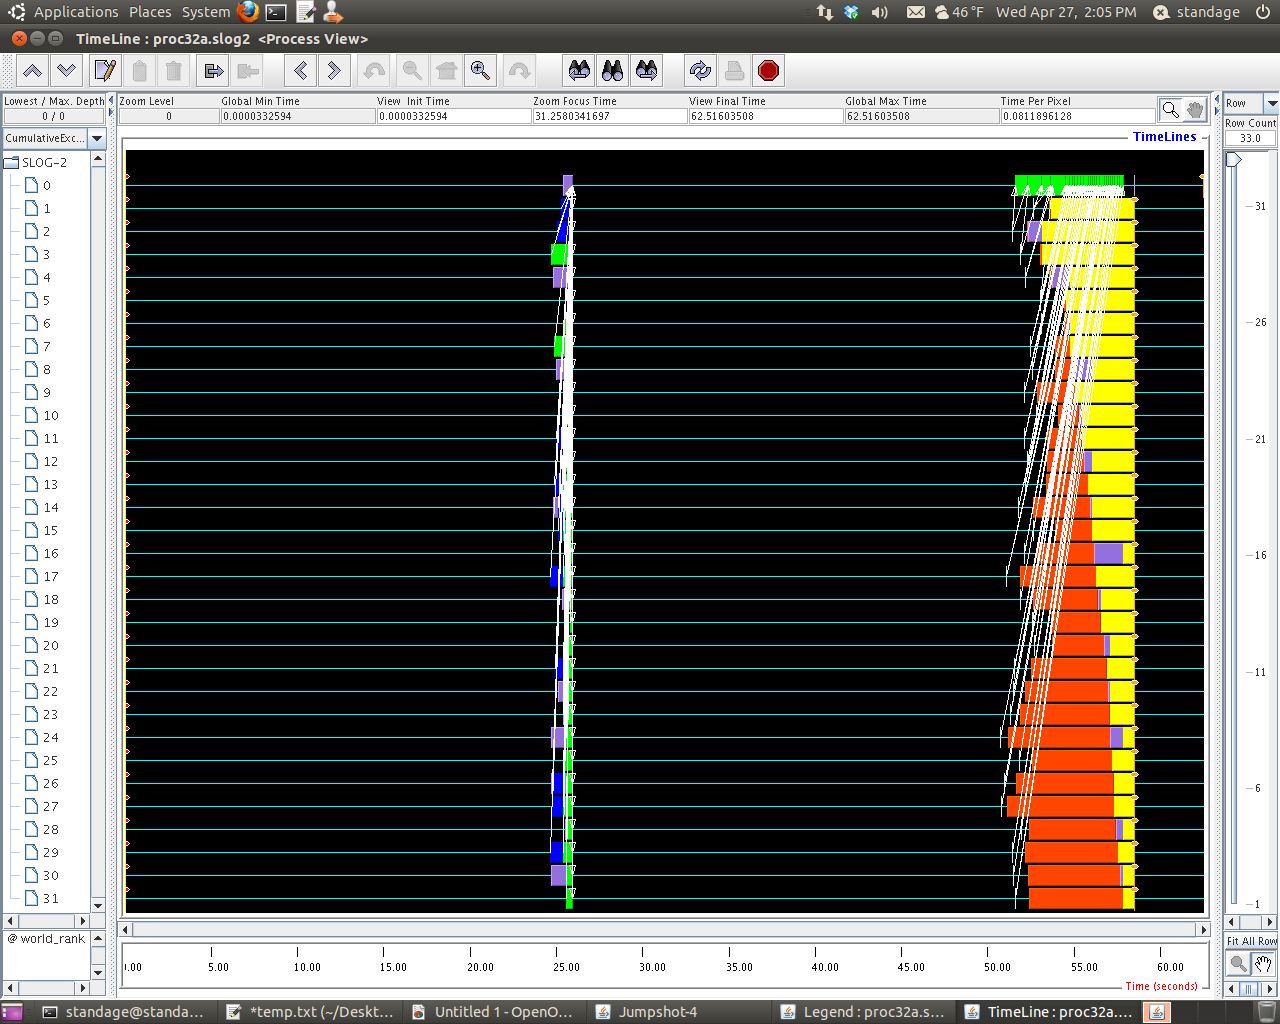
\includegraphics[height=200px]{proc32-hg.png}
  \end{center}
\end{frame}

\subsection{Scalability}
\begin{frame}
  \frametitle{Scalability}
  \begin{center}
    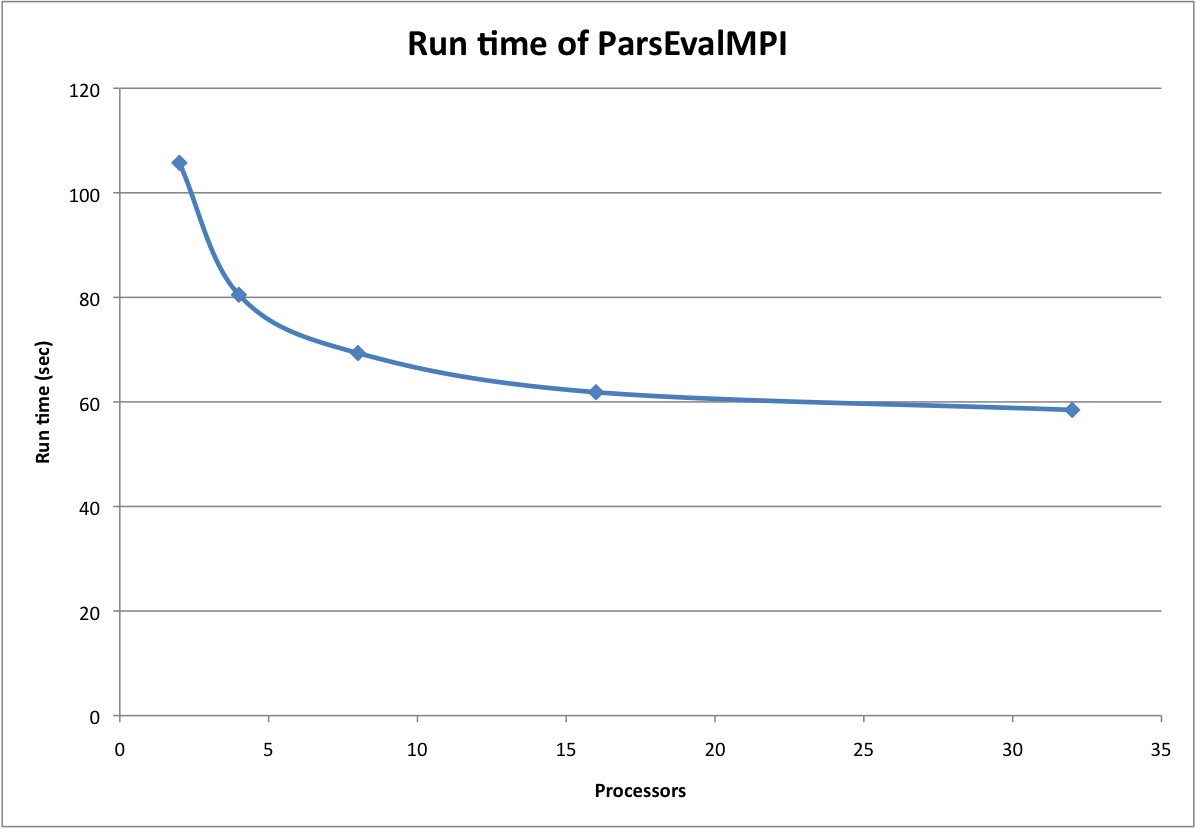
\includegraphics[height=200px]{runtime.png}
  \end{center}
\end{frame}
\begin{frame}
  \frametitle{Scalability}
  \begin{center}
    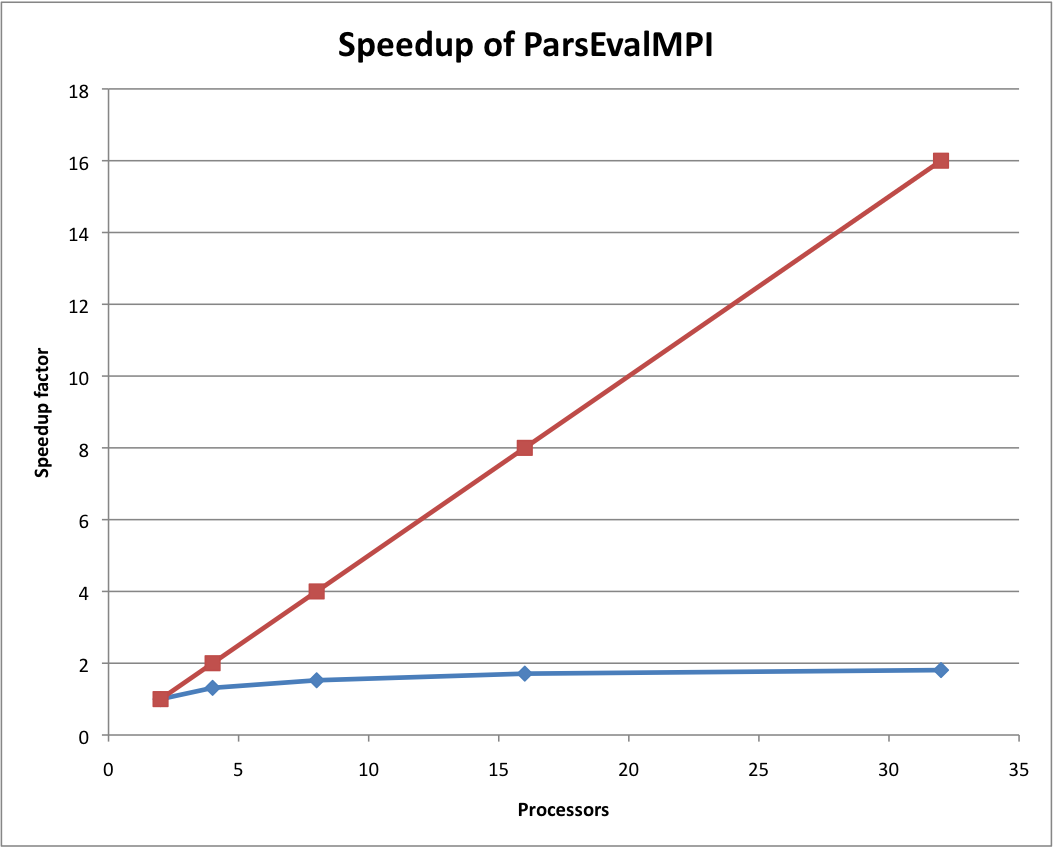
\includegraphics[height=200px]{speedup.png}
  \end{center}
\end{frame}

\subsection{Serial optimization}
\begin{frame}
  \frametitle{Serial optimization}
  \begin{itemize}
    \item<2-> Good
    \begin{itemize}
      \item<2-> native data types
      \item<2-> static arrays
    \end{itemize}
    \item<3-> Bad
    \begin{itemize}
      \item<3-> pointers, dynamic arrays
      \item<3-> dynamic data structures
    \end{itemize}
    \item<4-> Ugly
    \begin{itemize}
      \item<4-> copying data % different locations in memory, particularly bad stride access
      %\item<4-> calling \texttt{MPI\_Recv}'s in order
    \end{itemize}
  \end{itemize}
\end{frame}

\section{Conclusions}
\begin{frame}
  \frametitle{Conclusions}
  \begin{itemize}
    \item<2-> Excellent data distribution, load balancing
    \item<3-> Very poor scaling properties
    \begin{itemize}
      \item<4-> maximum scaling factor of 2?!?!
      \item<5-> perhaps try OpenMP
    \end{itemize}
    \item<6-> Significant improvement
  \end{itemize}
\end{frame}


\end{document}